\documentclass[11pt,a4paper]{article}
\usepackage[T1]{fontenc}
\usepackage{amsmath,amssymb,booktabs,graphicx}
\usepackage[margin=22mm]{geometry}

\setlength{\parindent}{0pt}
\setlength{\parskip}{5pt}
\setlength{\emergencystretch}{2em}
\newcommand{\E}{\mathbb{E}}
\newcommand{\unitsec}{\,\mathrm{s}}

\begin{document}

\begin{center}
{\large Modellierung \& Simulation I}\\[2mm]
{\Large Exercise 5 -- Problem 5.1}\\[1mm]
Group 40
\end{center}

\section*{1}

The simulator uses a first-come, first-served \(GI/GI/1\) queue with
unlimited waiting space. Since the queue starts empty, the first customers
tend to wait less than customers arriving during normal operation. We
therefore discard the first \(n_{\rm init}=10{,}000\) completed customers'
waiting times. Both this count and the batch length \(L=l_{\rm batch}\)
are configurable.

After warm-up, we collect complete batches and calculate the mean wait
\(\bar W\) and its 90\% confidence half-width \(h_W\). Starting with the
second batch, we check whether
\[
 h_W<0.0001\unitsec
 \qquad\text{or}\qquad
 \frac{h_W}{\bar W-h_W}<0.05.
\]
The relative condition is used only when \(\bar W>h_W\). Dividing by the
lower interval endpoint gives a conservative relative error. The absolute
condition allows the simulation to stop when the mean is close to zero.

\section*{3}

We fix the mean service time at \(1\unitsec\) and calculate the mean
interarrival time from the requested utilization,
\[
 \E[IAT]=\frac{\E[ST]}{\rho}=\frac{1}{\rho}\unitsec,
 \qquad 0.05\leq\rho\leq0.95.
\]
Service times are exponentially distributed. Interarrival times follow a
gamma distribution with shape \(1/c^2\) and scale \(c^2/\rho\unitsec\),
where \(c=\operatorname{cvar}[IAT]\). For \(c=0.5\), this is an Erlang-4
distribution. For \(c=1\), it is exponential. At \(c=2\), the gamma shape
is \(1/4\). This lets us compare different arrival variability at the
same average load.

\section*{4}

For each customer after warm-up, we record the wait \(W_i\) and the
indicator \(X_i=\mathbf{1}\{W_i>5\E[ST]\}\). Their averages estimate
\(\E[W]\) and \(p_{w,5}\), respectively. Since \(\E[ST]=1\unitsec\),
the excess probability is the fraction of customers who wait more than
five seconds.

We calculate a two-sided 90\% interval as
\[
 \bar Z\pm t_{0.95,m-1}\frac{s_Z}{\sqrt m}.
\]
For individual samples, \(Z\) is a waiting time or an exceedance indicator,
and \(m\) is the number of customers. For batch means, \(Z\) is the mean
wait or exceedance fraction within a batch, and \(m\) is the number of
batches. With complete batches of equal size, both calculations give the
same point estimate. Their interval widths differ because of the
dependence between consecutive waits. The supplied counter obtains the
\(t\) quantiles from an interpolated table.

\clearpage
\section*{5}

We use \texttt{DiscreteAutocorrelationCounter} to measure the lag-one
correlation of consecutive batch mean waits. The calibration covers all
57 combinations of utilization and interarrival CV. It uses fixed-length
runs and Lindley's waiting-time recursion with the same distributions
and time rounding as the event simulator.

\begin{center}
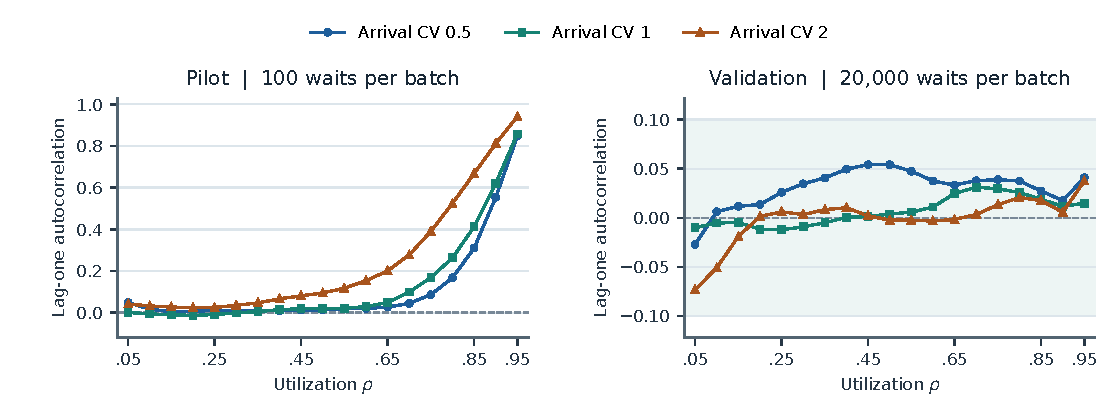
\includegraphics[width=\linewidth]{images/batch-autocorrelation.pdf}
\end{center}
{\small\textbf{Figure 1.} Lag-one autocorrelation for 100 and 20,000
waits per batch. The runs use 4,096 and 1,536 batches per setting,
respectively. The plots have different vertical scales. The shaded band
marks \(\lvert\widehat r(1)\rvert<0.10\).}

With 100 waits per batch, the correlation increases strongly at high
utilization. At \(\rho=0.90\), it is \(0.554\), \(0.621\), and \(0.811\)
for CVs \(0.5\), \(1\), and \(2\). At \(\rho=0.95\), these values rise
to \(0.847\), \(0.858\), and \(0.941\). The strongest correlation occurs
at \(\rho=0.95\) and CV \(=2\).

A busy server needs more time to clear a backlog, so successive batches
can be affected by the same queue. More variable arrivals create bursts
of customers, which makes this effect stronger. At low utilization,
idle periods let the queue empty more often.

Increasing the batch length to 20,000 lowers the correlation at
\((\rho,c)=(0.95,2)\) from \(0.941\) to \(0.037\). Across all validation
runs, the largest absolute value is \(0.073\), at \((0.05,2)\). We
therefore choose \(L=20{,}000\), using an absolute correlation below
\(0.10\) as our criterion. This checks adjacent batches at the tested
settings. It does not establish independence at every lag.

We use the longer calibration runs to assess the batch length because
the precision rule can stop after very few batches. In particular, the
centered lag-one estimator always returns \(-1\) for two different
batch means, making it uninformative in that case.

\clearpage
\section*{6}

For each setting, we discard 10,000 warm-up waits and collect 250 batches
of 20,000 waits. This gives five million measured waits per setting.
We use a fixed run length here because stopping as soon as the mean is
precise can leave too few observations of rare exceedances. The full
results and 90\% batch-means intervals are listed in the appendix.

\begin{center}
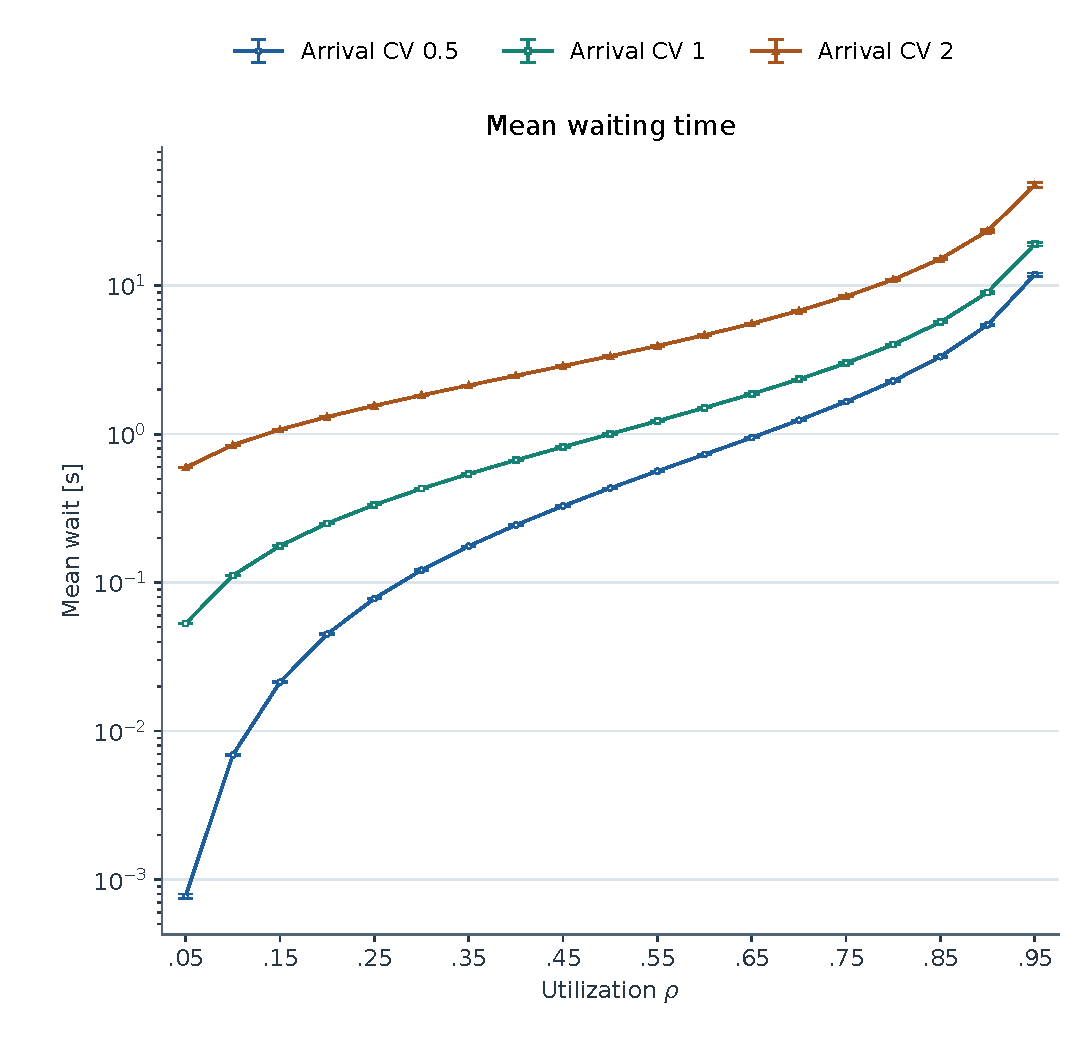
\includegraphics[width=\linewidth]{images/mean-wait-intervals.pdf}
\end{center}
{\small\textbf{Figure 2.} Mean waiting time in seconds with 90\%
batch-means confidence intervals. The vertical axis is logarithmic.}

\clearpage
\begin{center}
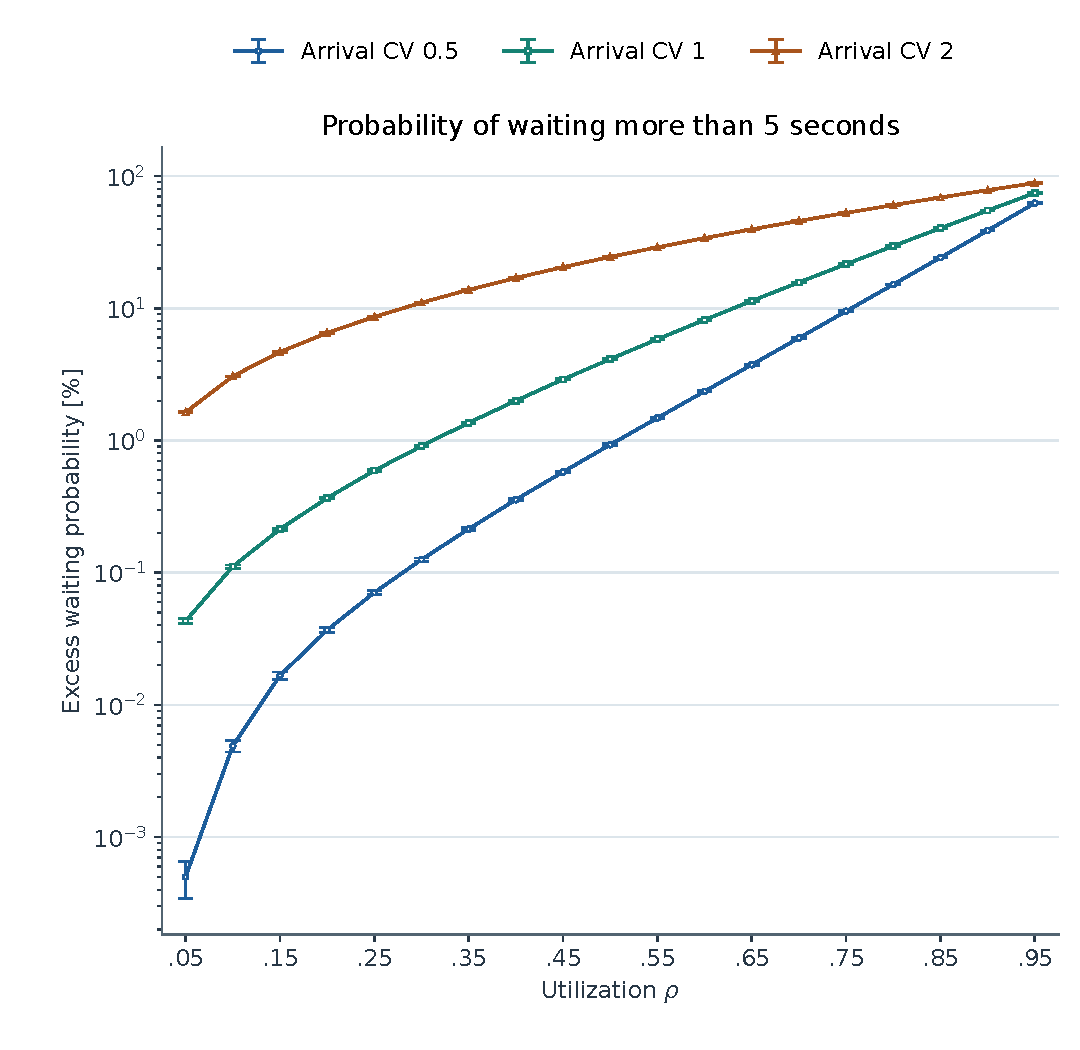
\includegraphics[width=\linewidth]{images/excess-probability-intervals.pdf}
\end{center}
{\small\textbf{Figure 3.} Probability of waiting more than five
seconds, expressed in percent, with 90\% batch-means confidence intervals.
The vertical axis is logarithmic.}

\clearpage
For CV \(=1\), increasing \(\rho\) from \(0.05\) to \(0.95\) raises the
mean wait from \(0.0530\unitsec\) to \(19.0448\unitsec\). The fraction
waiting more than five seconds increases from \(0.0430\%\) to
\(74.44\%\). Near capacity, the server has little spare time to clear
accumulated work. This explains why waiting times rise so steeply at
high utilization.

Arrival variability also has a large effect. At \(\rho=0.95\),
increasing the CV from \(0.5\) to \(2\) raises the mean from
\(11.91\unitsec\) to \(47.55\unitsec\), while the excess probability
rises from \(62.42\%\) to \(88.63\%\). Although the mean load is the
same, bursts of arrivals lead to much longer queues. The excess
probability shows how often the five-second limit is exceeded, which
cannot be read directly from the mean wait.

The least frequent exceedances occur at \((\rho,c)=(0.05,0.5)\). There
are only 25 in five million waits. The estimate is five per million,
with an interval of about 3.4 to 6.6 per million. The absolute
uncertainty is small, but the half-width is about \(32\%\) of the
estimate. More samples would be needed to estimate this small
probability with a low relative error.

\section*{7}

At \(\rho=0.95\), CV \(=2\), and \(L=20{,}000\), the precision rule
stops after 163 batches. This gives \(3{,}260{,}000\) measured waits,
or \(3{,}270{,}000\) completed customers including warm-up. The mean wait
is \(46.2726\unitsec\) and the excess probability is \(0.885976\).
The following intervals use the same observations.

\begin{center}
\small
\begin{tabular}{@{}llrr@{}}
\toprule
Quantity & Calculation & 90\% interval & Full width\\
\midrule
Mean wait (\(\mathrm{s}\)) & Batch means & \([44.0707,48.4745]\) & \(4.4038\)\\
Mean wait (\(\mathrm{s}\)) & Individual waits & \([46.2315,46.3138]\) & \(0.08230\)\\
\(p_{w,5}\) & Batch proportions & \([0.881872,0.890079]\) & \(0.008207\)\\
\(p_{w,5}\) & Individual indicators & \([0.885686,0.886265]\) & \(0.000579\)\\
\bottomrule
\end{tabular}
\end{center}

The batch-means interval for the mean wait is \(53.5\) times wider.
Its half-width is \(2.2019\unitsec\), giving a relative error of about
\(4.996\%\) under the stopping rule. Consecutive customers often wait
behind the same unfinished work, so their waiting times are positively
correlated. Treating these waits as independent ignores this covariance
and gives an interval that is too narrow. Exceedances also occur in
runs, so the same problem affects the probability interval.

\clearpage
\section*{8}

With \(L=1\), the simulation stops after just three measured waits,
or \(10{,}003\) completed customers including warm-up. Using the same
seeds gives a mean of \(73.1997\unitsec\) and a nominal 90\% interval
of \([70.5791,75.8202]\unitsec\). The apparent relative error is
\(3.71\%\).

These three customers arrive during a period with a large backlog and
have similar waiting times. Their small sample variance makes the
stopping rule declare sufficient precision far too early. The mean
therefore describes a short part of the queue trace. The longer run
with 20,000 waits per batch includes many more queue buildups and idle
periods and gives a better estimate of the steady-state mean.

For the chosen distributions, the continuous-time \(GI/M/1\) model
also gives a theoretical check. The root \(\sigma\in(0,1)\) satisfies
\[
 \sigma=\bigl(1+4(1-\sigma)/0.95\bigr)^{-1/4},
 \qquad \E[W]=\frac{\sigma}{1-\sigma}\unitsec.
\]
This gives \(\E[W]=48.4897\unitsec\). It is about \(0.015\unitsec\)
above the upper bound of the precision run's batch-means interval.
A 90\% interval can miss the true value in a particular run. At the
same setting, the five-million-sample run from Task 6 gives
\(47.5536\unitsec\) with interval
\([45.7406,49.3667]\unitsec\), which contains the theoretical value.
The batch-means results are therefore much more credible than the
estimate obtained from three correlated waits.

\clearpage
\section*{Appendix. Task 6 results}

Each cell contains an estimate and its 90\% batch-means interval.
The arrival and service seeds are 42 and 314159. Values with full
precision are stored in \texttt{task6-grid.csv} in Blatt 5.

\noindent\textbf{Mean waiting time (seconds)}
\par\nobreak\smallskip
{\centering\fontsize{8.1}{10.0}\selectfont
\begin{tabular*}{\linewidth}{@{\extracolsep{\fill}}rlll@{}}
\toprule
\(\rho\) & Arrival CV \(0.5\) & Arrival CV \(1\) & Arrival CV \(2\) \\
\midrule
0.05 & \(0.0007714\enspace[0.0007437,0.0007992]\) & \(0.05301\enspace[0.05274,0.05327]\) & \(0.5967\enspace[0.5952,0.5982]\) \\
0.10 & \(0.006896\enspace[0.006808,0.006984]\) & \(0.1117\enspace[0.1112,0.1121]\) & \(0.8448\enspace[0.8427,0.8470]\) \\
0.15 & \(0.02137\enspace[0.02120,0.02153]\) & \(0.1772\enspace[0.1765,0.1778]\) & \(1.075\enspace[1.072,1.078]\) \\
0.20 & \(0.04500\enspace[0.04474,0.04527]\) & \(0.2509\enspace[0.2500,0.2517]\) & \(1.308\enspace[1.305,1.312]\) \\
0.25 & \(0.07815\enspace[0.07775,0.07855]\) & \(0.3344\enspace[0.3332,0.3356]\) & \(1.556\enspace[1.552,1.561]\) \\
0.30 & \(0.1215\enspace[0.1210,0.1221]\) & \(0.4299\enspace[0.4284,0.4314]\) & \(1.829\enspace[1.823,1.834]\) \\
0.35 & \(0.1763\enspace[0.1756,0.1771]\) & \(0.5402\enspace[0.5383,0.5421]\) & \(2.134\enspace[2.126,2.141]\) \\
0.40 & \(0.2444\enspace[0.2434,0.2455]\) & \(0.6688\enspace[0.6664,0.6712]\) & \(2.481\enspace[2.471,2.490]\) \\
0.45 & \(0.3286\enspace[0.3273,0.3300]\) & \(0.8210\enspace[0.8179,0.8240]\) & \(2.883\enspace[2.871,2.895]\) \\
0.50 & \(0.4331\enspace[0.4313,0.4349]\) & \(1.004\enspace[0.9997,1.008]\) & \(3.360\enspace[3.345,3.376]\) \\
0.55 & \(0.5640\enspace[0.5616,0.5665]\) & \(1.227\enspace[1.222,1.232]\) & \(3.936\enspace[3.916,3.956]\) \\
0.60 & \(0.7308\enspace[0.7275,0.7341]\) & \(1.507\enspace[1.500,1.514]\) & \(4.648\enspace[4.622,4.674]\) \\
0.65 & \(0.9482\enspace[0.9436,0.9528]\) & \(1.866\enspace[1.856,1.876]\) & \(5.562\enspace[5.525,5.598]\) \\
0.70 & \(1.242\enspace[1.235,1.249]\) & \(2.344\enspace[2.331,2.358]\) & \(6.781\enspace[6.728,6.833]\) \\
0.75 & \(1.657\enspace[1.647,1.667]\) & \(3.012\enspace[2.992,3.032]\) & \(8.475\enspace[8.396,8.554]\) \\
0.80 & \(2.281\enspace[2.264,2.297]\) & \(4.015\enspace[3.983,4.047]\) & \(11.00\enspace[10.87,11.12]\) \\
0.85 & \(3.329\enspace[3.298,3.360]\) & \(5.687\enspace[5.631,5.744]\) & \(15.17\enspace[14.94,15.41]\) \\
0.90 & \(5.453\enspace[5.378,5.527]\) & \(9.023\enspace[8.893,9.153]\) & \(23.39\enspace[22.90,23.89]\) \\
0.95 & \(11.91\enspace[11.60,12.21]\) & \(19.04\enspace[18.53,19.56]\) & \(47.55\enspace[45.74,49.37]\) \\
\bottomrule
\end{tabular*}\par}

\medskip
\noindent\textbf{Probability of waiting more than five seconds (\%)}
\par\nobreak\smallskip
{\centering\fontsize{8.1}{10.0}\selectfont
\begin{tabular*}{\linewidth}{@{\extracolsep{\fill}}rlll@{}}
\toprule
\(\rho\) & Arrival CV \(0.5\) & Arrival CV \(1\) & Arrival CV \(2\) \\
\midrule
0.05 & \(0.0005000\enspace[0.0003422,0.0006578]\) & \(0.04302\enspace[0.04116,0.04488]\) & \(1.633\enspace[1.618,1.648]\) \\
0.10 & \(0.004900\enspace[0.004392,0.005408]\) & \(0.1114\enspace[0.1082,0.1147]\) & \(3.059\enspace[3.036,3.083]\) \\
0.15 & \(0.01668\enspace[0.01557,0.01779]\) & \(0.2135\enspace[0.2086,0.2185]\) & \(4.671\enspace[4.641,4.702]\) \\
0.20 & \(0.03684\enspace[0.03521,0.03847]\) & \(0.3669\enspace[0.3606,0.3733]\) & \(6.511\enspace[6.471,6.550]\) \\
0.25 & \(0.07074\enspace[0.06837,0.07311]\) & \(0.5920\enspace[0.5832,0.6008]\) & \(8.617\enspace[8.568,8.667]\) \\
0.30 & \(0.1257\enspace[0.1222,0.1291]\) & \(0.9066\enspace[0.8943,0.9188]\) & \(11.03\enspace[10.97,11.09]\) \\
0.35 & \(0.2141\enspace[0.2090,0.2191]\) & \(1.363\enspace[1.346,1.379]\) & \(13.81\enspace[13.74,13.88]\) \\
0.40 & \(0.3567\enspace[0.3494,0.3640]\) & \(1.999\enspace[1.976,2.021]\) & \(16.95\enspace[16.87,17.03]\) \\
0.45 & \(0.5784\enspace[0.5678,0.5891]\) & \(2.898\enspace[2.866,2.929]\) & \(20.49\enspace[20.39,20.59]\) \\
0.50 & \(0.9295\enspace[0.9141,0.9450]\) & \(4.130\enspace[4.087,4.172]\) & \(24.48\enspace[24.36,24.59]\) \\
0.55 & \(1.480\enspace[1.458,1.502]\) & \(5.829\enspace[5.773,5.886]\) & \(28.94\enspace[28.81,29.07]\) \\
0.60 & \(2.354\enspace[2.322,2.387]\) & \(8.174\enspace[8.099,8.249]\) & \(33.95\enspace[33.80,34.10]\) \\
0.65 & \(3.741\enspace[3.695,3.787]\) & \(11.37\enspace[11.27,11.47]\) & \(39.57\enspace[39.40,39.74]\) \\
0.70 & \(5.960\enspace[5.892,6.028]\) & \(15.70\enspace[15.57,15.82]\) & \(45.78\enspace[45.58,45.97]\) \\
0.75 & \(9.506\enspace[9.405,9.606]\) & \(21.59\enspace[21.43,21.75]\) & \(52.70\enspace[52.47,52.92]\) \\
0.80 & \(15.14\enspace[14.99,15.30]\) & \(29.58\enspace[29.37,29.78]\) & \(60.36\enspace[60.11,60.61]\) \\
0.85 & \(24.18\enspace[23.95,24.41]\) & \(40.39\enspace[40.11,40.66]\) & \(68.86\enspace[68.58,69.15]\) \\
0.90 & \(38.76\enspace[38.43,39.09]\) & \(54.91\enspace[54.55,55.27]\) & \(78.26\enspace[77.95,78.58]\) \\
0.95 & \(62.42\enspace[61.94,62.89]\) & \(74.44\enspace[73.98,74.91]\) & \(88.63\enspace[88.29,88.96]\) \\
\bottomrule
\end{tabular*}\par}


\end{document}
